% Provenance (never printed): see sources/outline_sources.md (Year 3:
% Glen's flow law; mass balance; ice sheets and ice shelves; sea ice;
% permafrost; the cryosphere's contribution to sea level).
% Brief: sources/book5/BRIEFS.md, ch. 24. Curves from figdata/bachelor-3/
% ice_flow.py (Glen slab, the plastic profile against the ETOPO1 Greenland
% transect, the Arkel ice cap) and sea_ice.py (NSIDC March and September
% extents, Stefan's law). Exercise and problem values in the Book 5 scratch
% calculator calc/ch24.py. The Arkel ice cap and the glaciers of the
% exercises are invented.
\chapter{Glaciologie}\label{ch:b3:glaciology}

Steek Groenland van west naar oost langs de breedtecirkel \ang{72.5}NB. Het ijs
begint enkele tientallen kilometers landinwaarts, stijgt steil, daarna steeds
vlakker, tot een brede top van \qty{3229}{m} hoogte, en daalt weer naar de bergen van de
oostkust. Uitgezet is het oppervlak nagenoeg een parabool die op zijn zij
ligt, met zijn top aan de rand. Dit hoofdstuk laat zien waar die vorm vandaan
komt: van een materiaal dat sneller en sneller kruipt naarmate het harder wordt
belast, zodat het zich bijna gedraagt alsof het niet meer dan een bepaalde spanning kan verdragen.
Daarna volgt het ijs van de sneeuw die het voedt tot de
zee die het ontvangt.
% ledger: data:b5-etopo-greenland

\begin{recall}
Gletsjers, ijskappen, ijsplaten, ijsbergen, zee-ijs, permafrost en de ijstijden
komen aan bod in de schoolboeken. Vloeiwetten en \omterm{def:b3:deformation-mechanisms:creep}{dislocatiekruip} staan in
Hoofdstuk~\ref{ch:b3:deformation-mechanisms}; \omterm{def:b3:gravity-geodesy:satgrav}{satellietgravimetrie} en de
massabalans van de ijskap die daarmee wordt gemeten in Hoofdstuk~\ref{ch:b3:gravity-geodesy};
ijskernen en hun zuurstofisotopen in Hoofdstuk~\ref{ch:b3:stable-isotopes}.
De zeeniveaubegroting, de ijs--albedoterugkoppeling en de thermosterische
zeeniveaustijging staan in Boek~4, in het hoofdstuk over antropogene
klimaatverandering. Latente warmte en warmtegeleiding staan in de natuurkundeboeken.
\end{recall}

\section{IJs als materiaal}\label{sec:b3:glaciology:material}

Gletsjerijs is een gesteente, een massa in elkaar grijpende ijskristallen, en het
vervormt dicht bij zijn smeltpunt. Onder spanning kruipt het door de
beweging van \omterm{def:b3:deformation-mechanisms:dislocation}{dislocaties} in zijn kristallen, net als de gesteenten uit
Hoofdstuk~\ref{ch:b3:deformation-mechanisms}, en zijn vloeiwet heeft dezelfde
vorm: een macht van de spanning maal een Arrhenius-factor.

\begin{theorem}[Glens vloeiwet]\label{thm:b3:glaciology:glen}
In isotroop gletsjerijs is de tensor van de reksnelheid evenredig met de
deviatorische spanning,
\[
\dot\varepsilon_{ij} = A(T)\,\tau_e^{\,n-1}\,\tau'_{ij}, \qquad
\tau_e^2 = \tfrac12\,\tau'_{ij}\tau'_{ij},
\]
met $n = 3$ en een \omterm{def:b3:glaciology:glen}{snelheidsfactor} $A(T)$ die toeneemt met de temperatuur. In
eenvoudige schuif, met $\tau_{xz}$ als enige niet-nulle deviatorische spanning, geldt
$\dot\varepsilon_{xz} = A\tau_{xz}^{\,n}$.
\end{theorem}
\index{Glens vloeiwet}

\begin{proof}
De wet zelf is empirisch: een machtswet die is gefit op kruipexperimenten en
op de vervorming van gletsjers, waarbij de coëfficiënt en de exponent
samen gefit. In eenvoudige schuif geldt $\tau'_{xz} = \tau'_{zx} = \tau_{xz}$ en de
overige componenten verdwijnen, dus $\tau_e^2 = \tfrac12(\tau_{xz}^2 +
\tau_{zx}^2) = \tau_{xz}^2$, en $\dot\varepsilon_{xz} = A\tau_{xz}^{\,n-1}
\tau_{xz}$.
\end{proof}
% ledger: pism:rheology

Bij $n = 3$ is ijs een sterk niet-lineaire vloeistof: verdubbelt de spanning, dan
vervormt het acht keer zo snel. De effectieve viscositeit, $1/(2A\tau_e^{\,2})$,
is geen eigenschap van het ijs alleen, maar neemt af naarmate de spanning stijgt.

\begin{definition}[Snelheidsfactor (ijs)]\label{def:b3:glaciology:glen}
De \emph{snelheidsfactor}\index{snelheidsfactor (ijs)} $A(T)$ van de vloeiwet van Glen, ook
de zachtheid van het ijs genoemd, wordt geschreven als $A = A_0\exp(-Q/RT)$, met
een activeringsenergie $Q$. Een veelgebruikte fit (Paterson en Budd) neemt $A_0 =
\qty{3.61e-13}{s^{-1}.Pa^{-3}}$ en $Q = \qty{60}{kJ/mol}$ onder
\qty{-10}{\celsius}, en $A_0 = \qty{1.73e3}{s^{-1}.Pa^{-3}}$ en $Q =
\qty{139}{kJ/mol}$ erboven, dichter bij het smeltpunt, waar het ijs
sneller verzacht met de temperatuur.
\end{definition}
% ledger: pism:rheology, codata:R

\begin{center}
\begin{tabular}{lccc}
\hline
temperatuur & \qty{-25}{\celsius} & \qty{-10}{\celsius} & \qty{0}{\celsius}\\
$A$ (\unit{Pa^{-3}.yr^{-1}}) & \num{2.7e-18} & \num{1.4e-17} & \num{1.4e-16}\\
\hline
\end{tabular}
\end{center}

IJs op zijn smeltpunt stroomt ongeveer vijftig keer zo snel als bij
\qty{-25}{\celsius} onder dezelfde spanning. Spanningen in gletsjers zijn van de
orde van een bar, \qty{e5}{Pa}.
% ledger: pism:rheology

Een gletsjer beweegt op twee manieren. Het ijs vervormt door kruip, overal; en
waar het bed op het smeltpunt zit, kan het ook glijden.

\begin{definition}[Basale glijding]\label{def:b3:glaciology:sliding}
\emph{Basale glijding}\index{basale glijding} is de beweging van een gletsjer over
zijn bed, op een dunne waterfilm of een laag zacht nat sediment. Dit
vereist een bed op het smeltpunt; een gletsjer die aan zijn bed is vastgevroren beweegt alleen
door het kruip van zijn ijs.
\end{definition}
% ledger: nsidc:glacier-flow

\section{Gletsjerstroming}\label{sec:b3:glaciology:flow}

\begin{theorem}[Stroming van een slab met evenwijdige zijden]\label{thm:b3:glaciology:slab}
Een slab van ijs met dikte $H$ en dichtheid $\rho$ ligt op een bed met helling
$\alpha$ en stroomt er langs af door eenvoudige schuif, glijdend met snelheid $u_b$. Op
hoogte $z$ boven het bed is de schuifspanning $\tau = \rho g(H - z)\sin\alpha$,
de snelheid
\[
u(z) = u_b + \frac{2A}{n + 1}(\rho g\sin\alpha)^n\left[H^{n+1} - (H -
z)^{n+1}\right],
\]
en de flux per eenheid van breedte $q = u_bH + \dfrac{2A}{n + 2}(\rho
g\sin\alpha)^nH^{n+2}$. De basale schuifspanning is $\tau_b = \rho gH\sin\alpha$.
\end{theorem}

\begin{proof}
Het ijs boven hoogte $z$ heeft per eenheid van oppervlak een gewicht $\rho g(H - z)$; zijn
component langs de helling, $\rho g(H - z)\sin\alpha$, wordt in evenwicht gehouden door de
schuifspanning op de onderkant, want het oppervlak is spanningsvrij. Volgens de wet van Glen
geldt $\mathrm du/\mathrm dz = 2\dot\varepsilon_{xz} = 2A\tau^n$; integreren vanaf
het bed, waar $u = u_b$, levert $u(z)$ op, en het integreren van $u$ van 0 tot $H$
levert $q$ op.
\end{proof}

De snelheid verandert weinig in het bovenste deel van de plaat en snel vlak bij het
bed, waar de spanning het grootst is: met $n = 3$ is de schuif geconcentreerd in
de onderste lagen. De oppervlaktesnelheid groeit als $H^{n+1} = H^4$ en als de
derde macht van de helling: een ijskap die twee keer zo dik is, stroomt zestien keer zo snel.

\begin{definition}[Ondiepe-ijsbenadering]\label{def:b3:glaciology:sia}
De \emph{ondiepe-ijsbenadering}\index{ondiepe-ijsbenadering} behandelt een ijskap waarvan de
dikte klein is ten opzichte van de breedte als plaatselijk een plaat met evenwijdige
zijden: op elke plek vervormt het ijs door eenvoudige schuif onder
de \emph{aandrijvende spanning} $\tau_d = \rho gH|\nabla s|$, waarbij $s$ de
oppervlaktehoogte is, en de flux volgt de plaatformule met de plaatselijke
dikte en oppervlaktehelling.
\end{definition}

In de \omterm{def:b3:glaciology:sia}{ondiepe-ijsbenadering} wordt de basale spanning bepaald door de vorm
van het ijs. Omdat de reksnelheid met de derde macht van de spanning toeneemt, geeft een
bescheiden toename van de spanning een grote toename van de stroming, die het ijs
dunner maakt en de spanning weer verlaagt: de spanning blijft binnen een smal bereik,
wat de omvang van de ijsmassa ook is. Trek dit door tot de limiet, een materiaal dat
vervormt helemaal niet onder een vloeigrens $\tau_0$ en vervormt zonder grens
boven die grens, dan volgt de vorm.

\begin{proposition}[Plastisch ijskapprofiel]\label{prop:b3:glaciology:nye}
Een perfect plastische ijskap met vloeigrens $\tau_0$ op een vlak horizontaal bed heeft, op
afstand $x$ landinwaarts van zijn rand, de oppervlaktehoogte
\[
h(x) = \sqrt{\frac{2\tau_0x}{\rho g}} .
\]
\end{proposition}
\index{plastisch ijskapprofiel}

\begin{proof}
Overal is de basale spanning gelijk aan de vloeigrens: $\rho gh\,\mathrm
dh/\mathrm dx = \tau_0$, waarbij de helling klein is. Dan is $\mathrm d(h^2)/\mathrm
dx = 2\tau_0/(\rho g)$, en $h = 0$ aan de rand.
\end{proof}

\begin{omfigure}
\begin{tikzpicture}
\begin{groupplot}[group style={group size=2 by 1, horizontal sep=1.5cm},
  height=0.4\linewidth,
  tick label style={font=\scriptsize}, label style={font=\small}, title style={font=\small}]
\nextgroupplot[width=0.38\linewidth, xlabel={$u/u_s$}, ylabel={hoogte boven het bed, $z/H$},
  xmin=0, xmax=1.05, ymin=0, ymax=1, title={een plaat},
  legend style={font=\scriptsize, at={(0.03,0.97)}, anchor=north west}]
% computed in figdata/bachelor-3/ice_flow.py
\addplot[omThm, thick] table[x=u3, y=zeta] {figdata/out/bachelor-3-ice_flow-slab.dat};
\addlegendentry{$n = 3$}
\addplot[omDef, thick, densely dashed] table[x=u1, y=zeta] {figdata/out/bachelor-3-ice_flow-slab.dat};
\addlegendentry{$n = 1$}
\addplot[omMeth, thick] table[x=u3b, y=zeta] {figdata/out/bachelor-3-ice_flow-slab.dat};
\addlegendentry{$n = 3$, glijdend}
\nextgroupplot[width=0.58\linewidth, xlabel={afstand vanaf \ang{58}~WL langs \ang{72.5}NB (\unit{km})},
  ylabel={hoogte (\unit{m})}, xmin=0, xmax=1270, ymin=-500, ymax=3700,
  title={Groenland}, scaled x ticks=false, xticklabel style={/pgf/number format/1000 sep={}},
  scaled y ticks=false, yticklabel style={/pgf/number format/1000 sep={}},
  legend style={font=\scriptsize, at={(0.5,0.03)}, anchor=south}]
\addplot[black, thin] table[x=x, y=h] {figdata/out/bachelor-3-ice_flow-gl.dat};
\addlegendentry{ijs- en landoppervlak}
\addplot[omThm, thick, densely dashed] table[x=x, y=h] {figdata/out/bachelor-3-ice_flow-nye-w.dat};
\addlegendentry{plastische profielen}
\addplot[omThm, thick, densely dashed, forget plot] table[x=x, y=h] {figdata/out/bachelor-3-ice_flow-nye-e.dat};
\draw[black!40] (axis cs:0,0) -- (axis cs:1270,0);
\node[font=\scriptsize, omThm, align=center] at (axis cs:330,2900) {$\tau_0 = $\\ \qty{72}{kPa}};
\node[font=\scriptsize, omThm, align=center] at (axis cs:1040,2900) {$\tau_0 = $\\ \qty{108}{kPa}};
\end{groupplot}
\end{tikzpicture}

\par\smallskip{\small Links, de snelheid over een plaat ijs, geschaald met de
oppervlaktesnelheid: de wet van Glen ($n = 3$) concentreert de schuif vlak bij het bed, een
lineaire vloeistof ($n = 1$) spreidt haar uit; met glijding wordt het hele profiel
verschoven. Rechts het oppervlak van Groenland langs \ang{72.5}NB (ETOPO1 Ice
Surface, NOAA NCEI), en de plastische profielen die aan de twee zijden ervan zijn gefit,
voor hoogten boven \qty{1000}{m} en een bed op zeeniveau. De fits vragen
vloeigrenzen van \qty{72}{kPa} en \qty{108}{kPa}, de orde van grootte van de bar bij
echte gletsjers; ze missen de steile randen, waar het bed en het smelten
een rol spelen.}\label{fig:b3:glaciology:flow}
\end{omfigure}
% ledger: data:b5-etopo-greenland, pism:rheology

\section{Massabalans}\label{sec:b3:glaciology:mass-balance}

Een gletsjer wordt gevoed door sneeuw en verliest ijs door smelten, verdamping en, waar hij
water bereikt, door afbreken.
% ledger: nsidc:glacier-zones

\begin{definition}[Massabalans; accumulatie- en ablatiezones; evenwichtslijn]\label{def:b3:glaciology:mass-balance}
De \emph{gletsjermassabalans}\index{gletsjermassabalans} is de verandering
van de massa van een gletsjer over een jaar, meestal uitgedrukt in meter
waterequivalent gemiddeld over zijn oppervlak. De
\emph{oppervlaktemassabalans}\index{oppervlaktemassabalans} is het deel dat te danken is aan de processen
aan het oppervlak, sneeuwval minus smelten, afvoer en sublimatie; de rest gaat verloren
door \omterm{def:b3:glaciology:grounding-line}{kalven} en door smelten aan de basis of onder drijvend ijs. De
\emph{accumulatiezone}\index{accumulatiezone} is het deel van het
oppervlak waar de oppervlaktemassabalans over een jaar positief is, de
\emph{ablatiezone}\index{ablatiezone} is het deel waar hij negatief is, en
de \emph{hoogte van de evenwichtslijn}\index{hoogte van de evenwichtslijn}
(ELA) is de hoogte van de lijn ertussen, waar hij nul is.
\end{definition}

\begin{omfigure}
\centering
\begin{tikzpicture}[>=stealth, font=\small, x=1cm, y=1cm]
% bed and surface of a valley glacier, long section
\fill[black!12] (0,0) -- (0,4.6) .. controls (2,3.6) and (6,1.4) .. (11,0) -- cycle;
\fill[omSea!45] (0,4.6) .. controls (2,3.6) and (6,1.4) .. (11,0)
  -- (11,0) .. controls (8,1.0) and (4,3.2) .. (0.6,5.4) -- (0,5.6) -- cycle;
\draw[thick, black!70] (0,4.6) .. controls (2,3.6) and (6,1.4) .. (11,0);
\draw[thick, omDef] (0,5.6) -- (0.6,5.4) .. controls (4,3.2) and (8,1.0) .. (11,0);
% equilibrium line
\draw[omThm, densely dashed, thick] (5.0,2.76) -- (5.0,4.6);
\node[omThm, font=\scriptsize, anchor=south] at (5.0,4.6) {evenwichtslijn (ELA)};
% balance arrows
\foreach \x/\y in {1.2/5.02, 2.4/4.27, 3.6/3.56} {\draw[->, omDef, thick] (\x,\y+0.55) -- (\x,\y+0.05);}
\foreach \x/\y in {6.4/2.02, 7.6/1.42, 8.8/0.86} {\draw[->, omThm, thick] (\x,\y+0.02) -- (\x,\y+0.52);}
\node[omDef, font=\scriptsize, align=center] at (2.4,6.2) {accumulatiezone:\\sneeuwwinst};
\node[omThm, font=\scriptsize, align=center] at (8.6,2.5) {ablatiezone:\\ijsverlies};
% flow lines, computed inside the ice: buried in the accumulation zone, emerging in the ablation zone
\draw[->, black!60] plot[smooth] coordinates {(1.00,5.14) (1.98,4.28) (2.95,3.54) (3.93,2.93) (4.90,2.43) (5.88,2.00) (6.85,1.62) (7.83,1.24) (8.80,0.86)};
\draw[->, black!60] plot[smooth] coordinates {(2.20,4.39) (2.84,3.89) (3.48,3.43) (4.11,3.02) (4.75,2.67) (5.39,2.36) (6.03,2.08) (6.66,1.82) (7.30,1.56)};
\draw[->, black!60] plot[smooth] coordinates {(3.40,3.67) (3.74,3.44) (4.08,3.21) (4.41,3.00) (4.75,2.81) (5.09,2.63) (5.42,2.47) (5.76,2.32) (6.10,2.17)};
\node[font=\scriptsize, anchor=north east] at (10.9,-0.1) {gletsjertong};
\node[font=\scriptsize] at (3.0,1.4) {vaste gesteente};
\end{tikzpicture}

\par\smallskip{\small Een schematische lange doorsnede van een dalgletsjer in
balans. Boven de evenwichtslijn wordt de sneeuw van elk jaar begraven en
meegevoerd de gletsjer in; eronder verliest het oppervlak elk jaar ijs en
wordt vernieuwd door ijs dat uit de diepte omhoogkomt. De stroomlijnen (grijs) dalen in de
\omterm{def:b3:glaciology:mass-balance}{accumulatiezone} en stijgen in de \omterm{def:b3:glaciology:mass-balance}{ablatiezone}; de stroming brengt het
overschot van de ene naar het tekort van de andere.}\label{fig:b3:glaciology:zones}
\end{omfigure}
% ledger: nsidc:glacier-zones, nsidc:glacier-flow

Op de ijskappen en de hoge gletsjers wordt sneeuw niet binnen één
seizoen tot ijs. Ze wordt door latere sneeuw bedekt, samengeperst en gerekristalliseerd.

\begin{definition}[Firn; poriënafsluiting]\label{def:b3:glaciology:firn}
\emph{Firn}\index{firn} is sneeuw die minstens één smeltseizoen heeft overleefd
en die tot ijs wordt samengeperst: dichter dan sneeuw, maar nog
doorlaatbaar voor lucht. \emph{Poriënafsluiting}\index{poriënafsluiting} is het punt in dat
verdichtingsproces, bij een dichtheid van ongeveer \qtyrange{820}{830}{kg/m^3}, waarop de
poriën tussen de korrels worden tot bellen afgesloten en de lucht erin wordt
afgesneden van de atmosfeer.
\end{definition}

Op de poolijskappen ligt de \omterm{def:b3:glaciology:firn}{poriënafsluiting} \qtyrange{50}{120}{m} onder het
oppervlak, afhankelijk van de temperatuur, de accumulatie en de
verontreinigingen; de lucht in de bellen van een ijskern is daarom jonger dan
het ijs eromheen, zoals Hoofdstuk~\ref{ch:b3:stable-isotopes} al ophaalde. Voor de
meeste gletsjers duurt de overgang van sneeuw naar ijs meer dan honderd jaar.
% ledger: nsidc:firn, firn:close-off

Een gletsjer reageert niet meteen op een verandering van zijn klimaat. Zijn
dikte moet eerst veranderen voordat zijn lengte kan volgen.

\begin{proposition}[Responstijd van de gletsjer]\label{prop:b3:glaciology:response}
Een gletsjer met typische dikte $H$ waarvan de \omterm{def:b3:glaciology:mass-balance}{gletsjermassabalans} aan het front $b_t <
0$ (in meter ijs per jaar) past zich aan een klimaatverandering aan in een tijd van de
orde van
\[
\tau = \frac{H}{-b_t} .
\]
\end{proposition}

\begin{proof}
Een verandering van de balans met $\delta b$ over de gletsjer verandert het volume
totdat het oppervlak dat aan het front verloren gaat of wordt gewonnen, waar de balans $b_t$ is,
compenseert dit: $L\,\delta b = -b_t\,\delta L$ per eenheid van breedte, voor een
gletsjer met lengte $L$. De benodigde volumeverandering is ongeveer $H\,\delta L$, en
de onbalans die dit aandrijft is aanvankelijk $L\,\delta b$ per jaar, zodat de
verandering $H\,\delta L/(L\,\delta b) = H/(-b_t)$ jaar duurt.
\end{proof}

Een gletsjer van \qty{200}{m} dik die bij zijn tong \qty{5}{m} ijs per jaar verliest
heeft ongeveer veertig jaar nodig om te reageren. Gletsjers hinken dus achter op het
klimaat: die van vandaag zullen decennia lang massa blijven verliezen, zelfs als de
temperatuur ophoudt te stijgen.
% ledger: ar6ch9:glaciers

\section{IJskappen en ijsplaten}\label{sec:b3:glaciology:ice-sheets}

De ijskappen van Groenland en Antarctica bevatten meer dan
\qty{99}{\percent} van het landijs. Die van Groenland beslaat \qty{1.7}{\mega
km^2} en is op de dikste plaatsen meer dan \qty{3}{km} dik; die van Antarctica
beslaat bijna \qty{14}{\mega km^2} en is op de dikste plaatsen bijna \qty{4.9}{km} dik. Veel
delen van de Antarctische ijskap rusten op een bodem onder het zeeniveau.
% ledger: nsidc:ice-sheets, ar6ch9:faq91

\begin{definition}[Ijsstroom]\label{def:b3:glaciology:ice-stream}
Een \emph{ijsstroom}\index{ijsstroom} is een band van een ijskap die veel sneller
stroomt dan het ijs aan weerszijden ervan, vooral door glijding of door de
vervorming van een zachte, natte bodem, en die een groot deel van het binnenland
van de ijskap naar de rand afvoert.
\end{definition}

\begin{definition}[Aardingslijn; kalven]\label{def:b3:glaciology:grounding-line}
De \emph{aardingslijn}\index{aardingslijn} is de lijn waar ijs dat op zijn bodem
rust en begint te drijven: zeewaarts ervan is het ijs een ijsplaat of een
drijvende gletsjertong. \emph{Kalven}\index{kalven} is het afbreken van
blokken ijs, ijsbergen, aan de voorkant van een gletsjer of een ijsplaat die
in water eindigt.
\end{definition}

IJsplaten drijven, dus hun smelten verhoogt het zeeniveau niet. Maar ze worden
aan hun zijkanten vastgehouden en op de heuvels van de zeebodem waar ze
aan de grond lopen, en de wrijving daar verzet zich tegen de stroming van het ijs
erachter: ze \emph{schragen} het. Nadat de ijsplaat Larsen~B in 2002 uiteenviel,
versnelden de gletsjers die er ijs naartoe hadden gevoerd, tot acht keer zo snel.
% ledger: nsidc:ice-shelves

\begin{proposition}[Drijfvermogen]\label{prop:b3:glaciology:flotation}
IJs met dichtheid $\rho_i$ en dikte $H$ op een bodem op diepte $D$ onder het zeeniveau,
in zeewater met dichtheid $\rho_w$, drijft als $H < (\rho_w/\rho_i)D$.
Met $\rho_i = \qty{917}{kg/m^3}$ en $\rho_w = \qty{1025}{kg/m^3}$ ligt de
\omterm{def:b3:glaciology:grounding-line}{aardingslijn} waar het ijs $1.12\,D$ dik is.
\end{proposition}

\begin{proof}
Drijvend ijs verdringt een gewicht water gelijk aan zijn eigen gewicht: een kolom met dikte $H$
heeft een diepgang $\rho_iH/\rho_w$ nodig. Als het water dieper is dan die diepgang,
drijft het ijs.
\end{proof}
% ledger: iapws:ice-density, noaa:seawater-1025

\begin{omfigure}
\centering
\begin{tikzpicture}[>=stealth, font=\small, x=1cm, y=1cm]
% sea and bed
\fill[omSea!50] (4.2,0) rectangle (11,-2.8);
\fill[black!15] (0,-0.9) -- (2.2,-2.0) -- (4.6,-1.6) -- (7.0,-2.3) -- (11,-2.6)
  -- (11,-3.2) -- (0,-3.2) -- cycle;
\draw[thick, black!60] (0,-0.9) -- (2.2,-2.0) -- (4.6,-1.6) -- (7.0,-2.3) -- (11,-2.6);
% grounded ice and ice shelf
\fill[white] (0,-0.9) -- (0,2.4) .. controls (2,2.2) and (3.6,1.4) .. (4.6,0.2)
  -- (9.2,0.12) -- (9.2,-1.0) -- (4.6,-1.6) -- (2.2,-2.0) -- cycle;
\draw[thick, omDef] (0,2.4) .. controls (2,2.2) and (3.6,1.4) .. (4.6,0.2) -- (9.2,0.12)
  -- (9.2,-1.0) -- (4.6,-1.6);
\draw[thick] (0,0) -- (0,0);
\draw[omDef!60, thin] (0,0) -- (4.3,0); \draw[omDef!60, thin] (9.2,0) -- (11,0);
\node[font=\scriptsize, anchor=south west] at (0.05,0.02) {zeeniveau};
% icebergs
\fill[white] (10.1,0.1) rectangle (10.6,-0.7); \draw[omDef] (10.1,0.1) rectangle (10.6,-0.7);
% labels
\fill[omThm] (4.6,-1.6) circle (0.07);
\draw[omThm, ->] (4.0,-2.6) node[anchor=north, font=\scriptsize] {aardingslijn} -- (4.55,-1.68);
\node[font=\scriptsize] at (1.4,1.1) {ijskap op de bodem};
\node[font=\scriptsize] at (6.9,-0.7) {drijvende ijsplaat};
\node[font=\scriptsize, anchor=south] at (9.2,0.2) {kalffront};
\node[font=\scriptsize, anchor=north, align=center] at (10.35,-0.8) {ijsberg};
\node[font=\scriptsize, align=center] at (2.1,-2.55) {bodem daalt\\landinwaarts};
\draw[->, black!60, thick] (2.2,1.6) -- (3.6,1.0);
\draw[->, black!60, thick] (5.4,-0.2) -- (7.0,-0.2);
\node[font=\scriptsize, align=center, omMeth] at (7.0,1.2) {schraging: wrijving aan de zijkanten\\en op de bodemrijzen van de ijsplaat};
\draw[->, omMeth, thick] (7.6,0.6) -- (6.6,0.6);
\end{tikzpicture}

\par\smallskip{\small Een schematische doorsnede van een mariene ijskap, niet op
schaal. Het ijs rust op een bodem onder het zeeniveau die landinwaarts dieper wordt; bij de
\omterm{def:b3:glaciology:grounding-line}{aardingslijn} begint het te drijven, als ijsplaat, die ijs verliest door
\omterm{def:b3:glaciology:grounding-line}{kalven} aan de voorkant en door smelten van onderaf. De wrijving op de plaat waar
die aan de zijkanten wordt vastgehouden en op bodemrijzen van de zeebodem verzet zich tegen de stroming van
het geaarde ijs.}\label{fig:b3:glaciology:grounding}
\end{omfigure}
% ledger: nsidc:ice-shelves, ar6ch9:misi

Op een bodem die landinwaarts dieper wordt, is de \omterm{def:b3:glaciology:grounding-line}{aardingslijn} kwetsbaar. Waar het
water dieper is, is het ijs bij de \omterm{def:b3:glaciology:grounding-line}{aardingslijn} dikker, volgens de drijfvoorwaarde,
en volgens de slabstelling neemt de stroom van een dikkere kolom
steil toe met de dikte. Als de \omterm{def:b3:glaciology:grounding-line}{aardingslijn} langs zo'n
helling terugtrekt, bereikt zij dikker ijs dat meer afvoert, sneller dunner wordt en
de lijn verder laat terugtrekken.

\begin{definition}[Instabiliteit van mariene ijskappen]\label{def:b3:glaciology:misi}
\emph{Instabiliteit van mariene ijskappen}\index{instabiliteit van mariene ijskappen}
(MISI) is de veronderstelde zichzelf versterkende terugtrekking van de
\omterm{def:b3:glaciology:grounding-line}{aardingslijn} van een ijskap die rust op een bodem die naar het binnenland
afloopt: zonder de tegenhouding door een ijsplaat is de \omterm{def:b3:glaciology:grounding-line}{aardingslijn} op zo'n
bodem inherent instabiel totdat zij een bodem bereikt die omhoog loopt.
\end{definition}

Ijsplaten kunnen een \omterm{def:b3:glaciology:grounding-line}{aardingslijn} ook op een dalende helling op zijn plaats houden.
Modellen waarin alle Antarctische ijsplaten worden weggehaald en niet mogen
hervormen, verliezen in 500 jaar via deze instabiliteit ijs dat \qtyrange{2}{10}{m}
\omterm{def:b3:glaciology:sle}{zeeniveau-equivalent} bedraagt, waarvan \qtyrange{2}{5}{m} uit West-Antarctica.
Bij ijskappen die grotendeels op vast gesteente boven het zeeniveau rusten, zoals
Groenland, is het belangrijkste zichzelf versterkende proces een ander: naarmate het oppervlak
smelt en daalt, ligt het in warmere lucht en smelt het meer.
% ledger: ar6ch9:misi, ar6ch9:faq91

\begin{definition}[Zeeniveau-equivalent]\label{def:b3:glaciology:sle}
Het \emph{zeeniveau-equivalent}\index{zeeniveau-equivalent} van een massa
landijs is de stijging van het mondiale gemiddelde zeeniveau die het smelten
ervan zou veroorzaken als het water zich over de huidige oceaan verspreidt.
\end{definition}

\begin{proposition}[Zeeniveau-equivalent van een massa ijs]\label{prop:b3:glaciology:sle}
Een massa $M$ ijs dat boven het zeeniveau rust, verspreid over een oceaan met oppervlakte
$A_o$ als water met dichtheid $\rho_w$, verhoogt het zeeniveau met $M/(\rho_wA_o)$:
ongeveer \qty{1}{mm} per \qty{360}{Gt}.
\end{proposition}

\begin{proof}
Het water beslaat het volume $M/\rho_w$ over het oppervlak $A_o$.
Met de \qty{360}{Gt} per millimeter die in de massabalansbeoordelingen van de
ijskappen wordt gehanteerd, geldt $A_o\rho_w = \qty{3.6e17}{kg/m}$: een oceaan van ongeveer
\qty{3.6e8}{km^2} voor water met de dichtheid van zoet water.
\end{proof}
% ledger: data:b5-imbie

Ijs dat al onder het zeeniveau ligt, verdringt zeewater en telt daarom minder mee:
het ijs van Antarctica, \qty{30}{\mega km^3}, komt overeen met ongeveer
\qty{58}{m} zeeniveau, minder dan de massa gedeeld door
\qty{360}{Gt/mm}.
% ledger: nsidc:ice-sheets

\begin{omfigure}
\centering
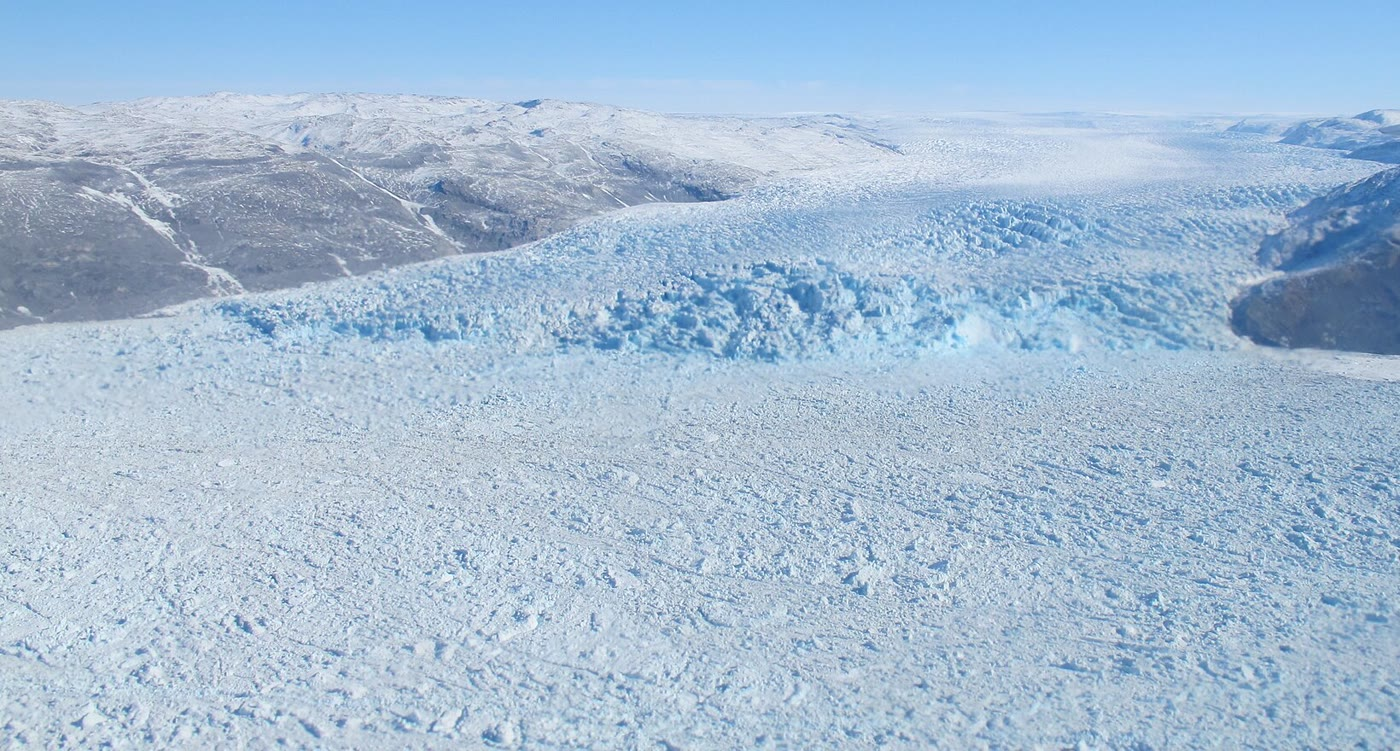
\includegraphics[width=0.82\linewidth]{images/book5/b3-greenland-outlet.jpg}

\par\smallskip{\small Een uitlaatgletsjer van de Groenlandse ijskap,
tussen bergen, die in zee eindigt bij zijn kalffront, de gebroken wand
van blauw ijs dwars door het midden van de foto; de fjord ervoor is volgepakt
met afgekalfd ijs en zee-ijs. Gefotografeerd vanuit een vliegtuig van NASA's
Operation IceBridge in april 2014 (NASA / Jim Yungel, publiek
domein).}\label{fig:b3:glaciology:outlet}
\end{omfigure}
% ledger: photo:b3-greenland-outlet

\begin{inthefield}[Een kamp op het ijs]
\begin{minipage}[t]{0.55\linewidth}\vspace{0pt}
Op een ijskap reizen de instrumenten van de glaciologen per slee en wonen zij
in tenten. Om te meten hoe snel het ijs beweegt, vriezen zij een paal in de
sneeuw en monteren zij daarop de antenne van een satellietnavigatieontvanger. De
ontvangers die in de geodesie worden gebruikt, leggen een positie vast tot binnen enkele centimeters, zodat
herhaalde posities over weken of seizoenen de snelheid en de richting van het ijs geven,
en de hoogte van de paal, opnieuw ingemeten, de uitdunning of aangroei
van het ijs eronder.
\end{minipage}\hfill
\begin{minipage}[t]{0.42\linewidth}\vspace{0pt}
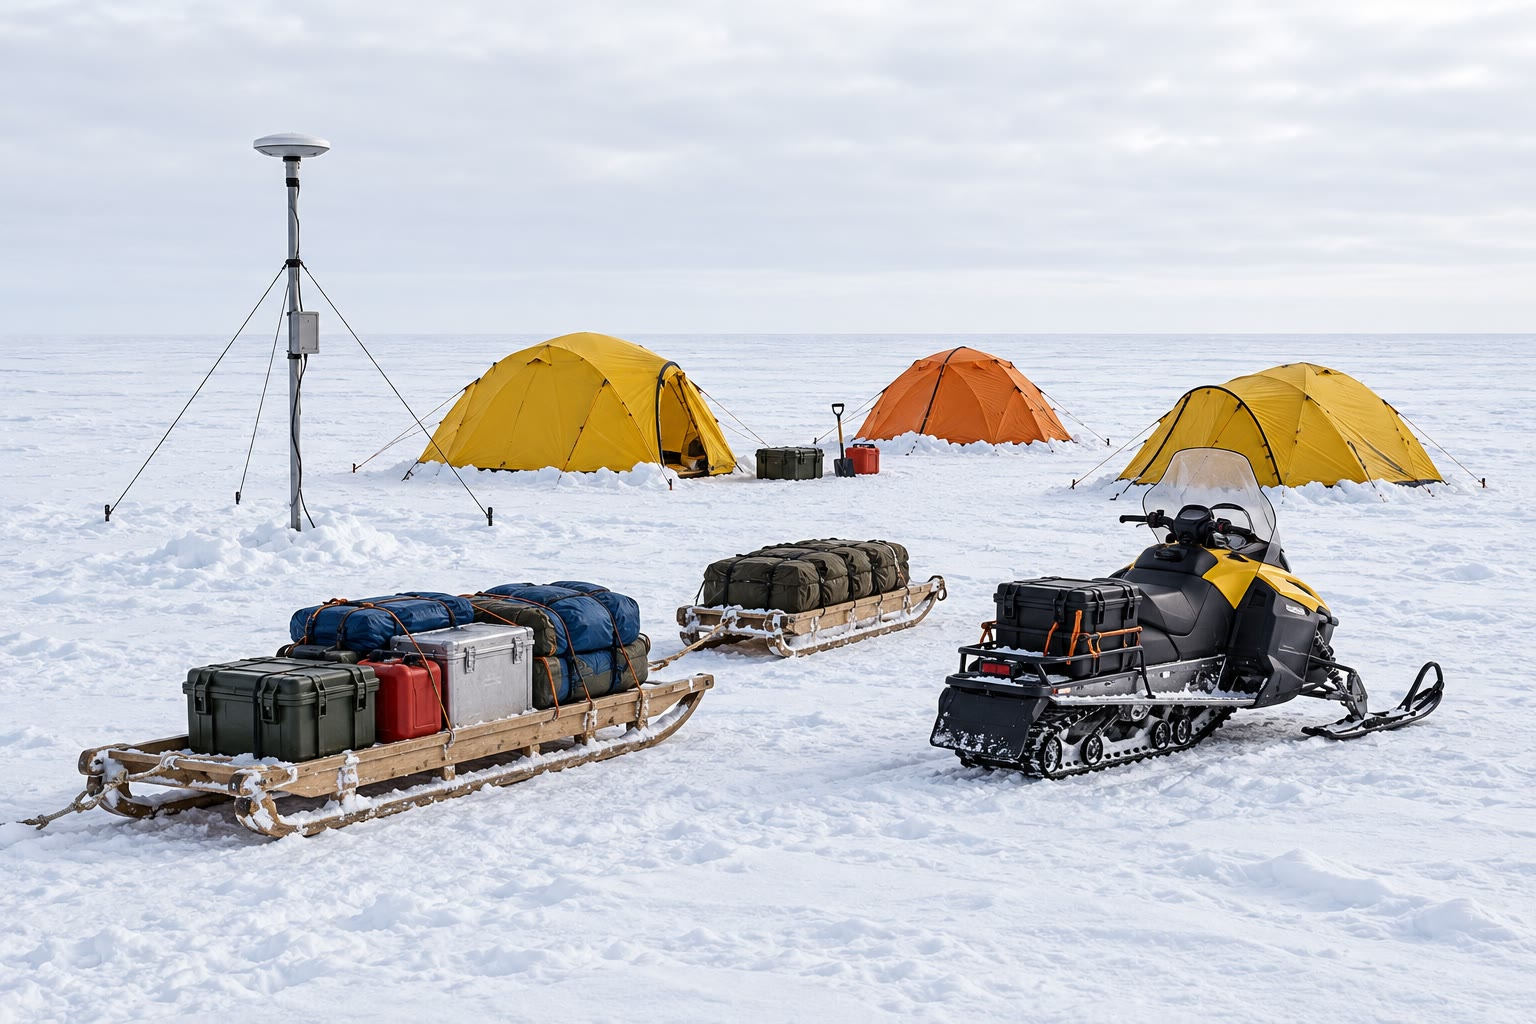
\includegraphics[width=\linewidth]{images/book5/ai/b3-glaciology-camp.jpg}

{\scriptsize Een veldkamp op een ijskap: tenten, sleeën en een
sneeuwscooter, en een satellietnavigatieantenne op een mast die wordt vastgehouden door
spanndraden (Door AI gegenereerde illustratie.)}.
\end{minipage}
\end{inthefield}
% ledger: gps:high-end

\section{Zee-ijs en permafrost}\label{sec:b3:glaciology:sea-ice}

Zee-ijs vormt zich, groeit en smelt in de oceaan. In de Arctis bereikt het zijn
grootste oppervlakte in maart en zijn kleinste in september.
% ledger: nsidc:sea-ice-def

\begin{definition}[Zee-ijsuitbreiding]\label{def:b3:glaciology:sea-ice}
De \emph{zee-ijsuitbreiding}\index{zee-ijsuitbreiding} is de totale oppervlakte van de
cellen van een satellietkaart waarin zee-ijs meer dan
\qty{15}{\percent} van het oppervlak bedekt. Zij is groter dan de zee-ijsoppervlakte,
die alleen het ijs zelf telt.
\end{definition}
% ledger: nsidc:sea-ice-def

Sinds satellieten het in 1979 begonnen te karteren, is de Arctische uitbreiding afgenomen, in
maart en veel sterker in september: met \qty{0.74}{\mega km^2} per decennium in
september, ongeveer \qty{12}{\percent} van het gemiddelde van 1981--2010 per decennium, tegenover
\qty{0.38}{\mega km^2}, \qty{2.5}{\percent}, in maart. De kleinste
uitbreiding in september tot nu toe, \qty{3.57}{\mega km^2}, was in 2012. Arctisch zee-ijs
weerkaatst \qtyrange{50}{70}{\percent} van het zonlicht, de open oceaan
ongeveer \qty{6}{\percent}: door het verlies van het ijs wordt het oppervlak donkerder, de ijs--albedoterugkoppeling
uit Boek~4.
% ledger: data:b5-nsidc-extent, nsidc:sea-ice-reflect

Zee-ijs groeit aan de onderkant, waar het zeewater erop bevriest, en de latente
warmte van dat bevriezen moet via het ijs omhoog naar de koude lucht worden geleid.

\begin{theorem}[Wet van Stefan]\label{thm:b3:glaciology:stefan}
Zee-ijs met warmtegeleidingscoëfficiënt $k_i$, dichtheid $\rho_i$ en latente
smeltwarmte $L$, waarvan het oppervlak op een temperatuur $\Delta T$ onder het
vriespunt van het water eronder wordt gehouden, groeit, als de warmte uit de
oceaan verwaarloosbaar is, volgens
\[
h(t)^2 - h(0)^2 = \frac{2k_i\,\Delta T}{\rho_iL}\,t .
\]
Onder een sneeuwlaag met dikte $h_s$ en geleidingsvermogen $k_s$ is de groeisnelheid
$\mathrm dh/\mathrm dt = \Delta T/[\rho_iL(h/k_i + h_s/k_s)]$.
\end{theorem}

\begin{proof}
De temperatuur in het dunne ijs is lineair, van het vriespunt aan de onderkant tot
de oppervlaktetemperatuur aan de bovenkant, dus de warmteflux erdoor is
$k_i\Delta T/h$, of, door ijs en sneeuw in serie, $\Delta T/(h/k_i +
h_s/k_s)$. Bij het bevriezen van een laag $\mathrm dh$ komt $\rho_iL\,\mathrm dh$ per
eenheid van oppervlak vrij, wat deze flux moet afvoeren: $\rho_iL\,\mathrm dh/\mathrm dt
= k_i\Delta T/h$. Dan geldt $\mathrm d(h^2)/\mathrm dt = 2k_i\Delta T/(\rho_iL)$.
\end{proof}

Met $k_i = \qty{2.03}{W.m^{-1}.K^{-1}}$, $L = \qty{3.34e5}{J/kg}$ en
$\rho_i = \qty{917}{kg/m^3}$ groeit een oppervlak dat \qty{20}{K} onder het
vriespunt ligt in honderd dagen \qty{1.5}{m} ijs en in tweehonderd dagen \qty{2.1}{m}.
Sneeuw, met een geleidingsvermogen van \qty{0.30}{W.m^{-1}.K^{-1}}, is een goede
isolator: \qty{20}{cm} ervan halveert de groei meer dan. Dik ijs groeit
langzaam, dun ijs snel: de wet heeft de neiging de dikte van het ijs na een
zomer van smelten weer gelijk te maken.
% ledger: cice:constants, iapws:ice-density

\begin{omfigure}
\begin{tikzpicture}
\begin{groupplot}[group style={group size=2 by 1, horizontal sep=1.5cm},
  width=0.48\linewidth, height=0.4\linewidth,
  tick label style={font=\scriptsize}, label style={font=\small}, title style={font=\small}]
\nextgroupplot[xlabel={jaar}, ylabel={uitbreiding (\unit{\mega km^2})}, xmin=1977, xmax=2028,
  ymin=0, ymax=18, title={Arctische zee-ijsuitbreiding},
  xticklabel style={/pgf/number format/1000 sep={}},
  legend style={font=\scriptsize, at={(0.03,0.66)}, anchor=west}]
% computed in figdata/bachelor-3/sea_ice.py
\addplot[omDef, thick, mark=*, mark size=0.9pt] table[x=year, y=mar] {figdata/out/bachelor-3-sea_ice-extent.dat};
\addlegendentry{maart}
\addplot[omThm, thick, mark=*, mark size=0.9pt] table[x=year, y=sep] {figdata/out/bachelor-3-sea_ice-extent.dat};
\addlegendentry{september}
\addplot[black!60, densely dashed, forget plot] table[x=year, y=mar] {figdata/out/bachelor-3-sea_ice-trend.dat};
\addplot[black!60, densely dashed, forget plot] table[x=year, y=sep] {figdata/out/bachelor-3-sea_ice-trend.dat};
\nextgroupplot[xlabel={dagen van vriezen}, ylabel={ijsdikte (\unit{m})}, xmin=0, xmax=200,
  ymin=0, ymax=2.4, title={groei, $\Delta T = \qty{20}{K}$},
  legend style={font=\scriptsize, at={(0.97,0.03)}, anchor=south east}]
\addplot[omMeth, thick] table[x=day, y=h0] {figdata/out/bachelor-3-sea_ice-stefan.dat};
\addlegendentry{kaal ijs}
\addplot[omDef, thick, densely dashed] table[x=day, y=hs] {figdata/out/bachelor-3-sea_ice-stefan.dat};
\addlegendentry{onder \qty{20}{cm} sneeuw}
\end{groupplot}
\end{tikzpicture}

\par\smallskip{\small Links, de gemiddelde Arctische \omterm{def:b3:glaciology:sea-ice}{zee-ijsuitbreiding} in maart en in
september, 1979--2026 (NSIDC Sea Ice Index, versie~4), met trends volgens de
kleinste kwadraten (gestreept): \qty{-0.38}{\mega km^2} en \qty{-0.74}{\mega km^2} per
decennium. Rechts, de groei van zee-ijs door geleiding onder een oppervlak dat
\qty{20}{K} onder het vriespunt ligt, zonder warmte uit de oceaan: kaal ijs volgens
de wet van Stefan, en hetzelfde ijs onder \qty{20}{cm} sneeuw.}\label{fig:b3:glaciology:sea-ice}
\end{omfigure}
% ledger: data:b5-nsidc-extent, cice:constants

Permafrost is grond die twee jaar of langer op of onder \qty{0}{\celsius} blijft.
Het ligt onder ongeveer een kwart van het ontoonde land van het noordelijk halfrond.
Hemisphere.
% ledger: nsidc:permafrost

\begin{definition}[Actieve laag]\label{def:b3:glaciology:permafrost}
De \emph{actieve laag}\index{actieve laag} is de laag grond boven de permafrost die
elke zomer ontdooit en elke winter opnieuw bevriest.
\end{definition}

De dikte ervan wordt, net als de groei van zee-ijs, bepaald door de geleiding van
warmte de grond in tijdens het ontdooiseizoen, tegenover de latente warmte van het
ijs in de grond. De temperatuur van de permafrost is de afgelopen drie tot vier
decennia overal in de permafrostgebieden gestegen (hoge betrouwbaarheid);
de permafrost is wereldwijd met \qty{0.29}{\celsius} [\numrange{0.17}{0.41}]
opgewarmd tussen 2007 en 2016 (gemiddelde betrouwbaarheid), en een toename van de
dikte van de \omterm{def:b3:glaciology:permafrost}{actieve laag} is een fenomeen over het hele Arctische gebied (gemiddelde betrouwbaarheid).
Waar het ijs erin smelt, kan de grond instorten.
% ledger: ar6ch9:permafrost, nsidc:permafrost-thaw

\section{De cryosfeer en het zeeniveau}\label{sec:b3:glaciology:sea-level}

Het budget van het zeeniveau uit Boek~4 telt de uitzetting van de opwarmende
oceaan op bij het water dat door het ijs en door het land wordt toegevoegd. Van de
\qty{3.69}{mm/yr} zeeniveaustijging die tussen 2006 en 2018 is waargenomen, droegen
gletsjers \qty{0.62}{mm/yr} bij, Groenland \qty{0.63}{mm/yr} en Antarctica
\qty{0.37}{mm/yr}: het ijs samen meer dan de uitzetting van de oceaan,
\qty{1.39}{mm/yr}.
% ledger: ar6ch9:table95

\begin{dated}{2021}
Groenland verloor \qty{4890}{Gt} aan ijs over 1992--2020 [4140 tot 5640],
\qty{13.5}{mm} zeeniveau, met snelheden die stegen van \qty{39}{Gt/yr} in de
jaren 1990 tot \qty{243}{Gt/yr} in 2010--2019, door afvoer en, in toenemende mate,
door oppervlaktesmelt (hoge betrouwbaarheid). Antarctica verloor \qty{2670}{Gt}
[1800 tot 3540], \qty{7.4}{mm}, met een snelheid die steeg van \qty{49}{Gt/yr} in de
jaren 1990 tot \qty{148}{Gt/yr} in 2010--2019; het verlies kwam van de uitlaatgletsjers van
West-Antarctica, vooral door het smelten van de ijsplaten van onderaf (hoge
betrouwbaarheid). De gletsjers buiten de ijskappen verloren \qty{6200}{Gt} over
1993--2019, \qty{17.1}{mm}, meer in 2010--2019 dan in welke andere decennium van de
reeks ook (zeer hoge betrouwbaarheid). Groenland zal deze eeuw onder alle beschouwde
scenario's blijven verliezen aan massa (vrijwel zeker), en Antarctica zal dat ook
doen (waarschijnlijk): tegen 2100 voegt Groenland waarschijnlijk
\qtyrange{0.01}{0.10}{m} toe aan het zeeniveau onder een scenario met lage emissies
en \qtyrange{0.09}{0.18}{m} onder een zeer hoog scenario, Antarctica
\qtyrange{0.03}{0.27}{m} en \qtyrange{0.03}{0.34}{m}. De Arctische Oceaan
zal waarschijnlijk praktisch vrij van zee-ijs worden, met minder dan
\qty{1}{\mega km^2} ervan, in zijn septemberminimum voor de eerste keer
vóór 2050 onder alle beschouwde scenario's.
\end{dated}
% ledger: ar6ch9:greenland, ar6ch9:antarctica, ar6ch9:glaciers, ar6ch9:ice-sheet-proj, ar6ch9:sea-ice

De verliezen van de ijskappen zijn die van Hoofdstuk~\ref{ch:b3:gravity-geodesy},
gemeten met altimetrie, met gravimetrie en met het verschil tussen de sneeuw
die valt en het ijs dat afstroomt: drie onafhankelijke methoden samengebracht
tot één schatting.
% ledger: data:b5-imbie

\section{Oefeningen}

\begin{exercise}[$\star$]\label{exo:b3:glaciology:1}
Een dalgletsjer van \qty{250}{m} dik stroomt af over een helling van \ang{3}. Bereken
de basale schuifspanning, en vergelijk die met de basale spanningen van echte
gletsjers, van de orde van een bar.
\end{exercise}

\begin{exercise}[$\star$]\label{exo:b3:glaciology:2}
(a)~De ijskap van Groenland bevat ongeveer \qty{2.9}{\mega km^3} ijs met
een dichtheid van \qty{917}{kg/m^3}. Bereken de massa en het \omterm{def:b3:glaciology:sle}{zeeniveau-equivalent} bij
\qty{360}{Gt/mm}, en vergelijk met de \qty{7.4}{m} die gewoonlijk wordt genoemd.
(b)~Doe hetzelfde voor de \qty{30}{\mega km^3} van Antarctica, opgegeven als ongeveer
\qty{58}{m}. Waarom verschillen de twee zo sterk?
\end{exercise}
% ledger: nsidc:ice-sheets

\begin{exercise}[$\star$]\label{exo:b3:glaciology:3}
Een gletsjer heeft een \omterm{def:b3:glaciology:mass-balance}{accumulatiezone} van \qty{6}{km^2} met een gemiddelde balans van
\qty{+1.2}{m} waterequivalent, en een \omterm{def:b3:glaciology:mass-balance}{ablatiezone} van \qty{4}{km^2} met
\qty{-2.1}{m}. Bereken de nettobalans in kubieke meter water, de gemiddelde
specifieke balans, en de accumulatiegebiedsverhouding. Groeit hij of
krimpt hij?
\end{exercise}

\begin{exercise}[$\star$]\label{exo:b3:glaciology:4}
Bij \omterm{def:b3:glaciology:firn}{poriënafsluiting} heeft het \omterm{def:b3:glaciology:firn}{firn} een dichtheid van \qtyrange{820}{830}{kg/m^3}.
Welk deel van zijn volume is nog poriënruimte (ijs:
\qty{917}{kg/m^3})?
\end{exercise}
% ledger: firn:close-off

\begin{exercise}[$\star\star$]\label{exo:b3:glaciology:5}
Een temperate gletsjer (ijs op \qty{0}{\celsius}, $A =
\qty{1.4e-16}{Pa^{-3}.yr^{-1}}$) is \qty{300}{m} dik op een helling van
\ang{3}. Bereken de oppervlaktesnelheid uitsluitend door interne vervorming. Met welke
factor verandert de snelheid als de gletsjer twee keer zo dik zou zijn? Als de helling
zou worden gehalveerd?
\end{exercise}

\begin{exercise}[$\star\star$]\label{exo:b3:glaciology:6}
Bereken uit de constanten van Paterson--Budd de \omterm{def:b3:glaciology:glen}{snelheidsfactor} bij
\qty{-25}{\celsius} en \qty{-10}{\celsius}, en de verhouding van de snelheden van
twee identieke ijsmassa's bij \qty{0}{\celsius} en bij \qty{-25}{\celsius}.
\end{exercise}
% ledger: pism:rheology, codata:R

\begin{exercise}[$\star\star$]\label{exo:b3:glaciology:7}
Bereken de grootste dikte van een plastische ijskap met een afstand van \qty{1000}{km}
van het midden tot de rand, met $\tau_0 = \qty{100}{kPa}$, en vergelijk die met de
grootste dikte van het Antarctische ijs, bijna \qty{4.9}{km}.
\end{exercise}
% ledger: nsidc:ice-sheets

\begin{exercise}[$\star\star$]\label{exo:b3:glaciology:8}
Een gletsjer van \qty{200}{m} dik verliest \qty{5}{m} ijs per jaar aan zijn tong.
Schat de responstijd. Stel dat het klimaat plotseling opwarmt en daarna constant blijft;
hoe lang blijft zijn lengte dan veranderen?
\end{exercise}

\begin{exercise}[$\star\star$]\label{exo:b3:glaciology:9}
(a)~Gebruik de wet van Stefan met $\Delta T = \qty{20}{K}$ en bereken de dikte
van kaal zee-ijs na 100 dagen, en de tijd die nodig is om \qty{3}{m} te bereiken.
(b)~Wat suggereert dit over ijs dat dikker is dan \qty{3}{m}?
\end{exercise}
% ledger: cice:constants

\begin{exercise}[$\star\star\star$]\label{exo:b3:glaciology:10}
(a)~Waar het bed \qty{800}{m} onder het zeeniveau ligt, hoe dik is het ijs bij
de \omterm{def:b3:glaciology:grounding-line}{aardingslijn}? (b)~Gebruik de slabflux $q \propto H^{n+2}$ bij een gegeven
oppervlaktehelling: met welke factor stijgt de flux van het geaarde ijs als de
\omterm{def:b3:glaciology:grounding-line}{aardingslijn} terugtrekt naar de plek waar het bed \qty{900}{m} diep is? (c)~Verklaar
waarom een bed dat landinwaarts dieper wordt de terugtrekking zelfversterkend maakt, en wat een
ijsplaat verandert.
\end{exercise}
% ledger: iapws:ice-density, noaa:seawater-1025

\begin{exercise}[$\star\star\star$]\label{exo:b3:glaciology:11}
Toon aan dat het volume van een cirkelvormige plastische ijskap met straal $R$ gelijk is aan $V =
\frac{8\pi}{15}\sqrt{2\tau_0/(\rho g)}\,R^{5/2}$. Met welke factor groeit het
\omterm{def:b3:glaciology:sle}{zeeniveau-equivalent} als de straal verdubbelt?
\end{exercise}

\begin{exercise}[$\star\star\star$]\label{exo:b3:glaciology:12}
De gemiddelde \omterm{def:b3:glaciology:sea-ice}{zee-ijsuitbreiding} in de Arctis was \qty{16.34}{\mega km^2} in maart 1979 en
\qty{14.13}{\mega km^2} in maart 2026; in september \num{7.05} en
\qty{4.81}{\mega km^2}. (a)~Bereken de relatieve verandering in elke maand.
(b)~Geef twee fysische redenen waarom de uitbreiding in september zoveel sneller is gedaald
dan die in maart.
\end{exercise}
% ledger: data:b5-nsidc-extent

\section{Probleem: de Arkel-ijskap}

\begin{problem}[{Weekendprobleem --- de vorm, stroming, massabalans en
zeeniveau-equivalent van een verzonnen ijskap}]
\label{pb:b3:glaciology:1}
De verzonnen Arkel-ijskap ligt op een vlak plateau. Hij is bijna cirkelvormig,
\qty{20}{km} in straal, en het ijs is op ongeveer \qty{-10}{\celsius}. Neem
$\rho = \qty{917}{kg/m^3}$ en $g = \qty{9.81}{m/s^2}$.

\medskip\noindent\textbf{Deel I --- Is de kap plastisch?}
\begin{enumerate}
\item Toon aan dat onder ijs met dikte $H$ en een kleine oppervlaktehelling
  $\alpha$ de basale schuifspanning ongeveer $\rho gH\alpha$ bedraagt.
\item Radarsondages en metingen op 5, 10 en \qty{15}{km} van het midden
  geven dikten van 580, 470 en \qty{335}{m} en oppervlaktehellingen van
  \num{0.0190}, \num{0.0240} en \num{0.0330}. Bereken de basale
  schuifspanning op de drie punten.
\item Is de kap dicht bij plastisch? Welke vloeispanning wordt aangenomen?
\item Met $\tau_0 = \qty{100}{kPa}$ bereken $2\tau_0/(\rho g)$.
\item Voorspel de dikte op de drie punten uit het plastische profiel
  en vergelijk die met de radarsondages.
\end{enumerate}

\medskip\noindent\textbf{Deel II --- Vorm en volume.}
\begin{enumerate}[resume]
\item Bereken de dikte in het midden.
\item Toon aan dat voor het volume geldt $V = \frac{8\pi}{15}\sqrt{2\tau_0/(\rho
  g)}\,R^{5/2}$.
\item Bereken het volume in kubieke kilometer.
\item Bereken het oppervlak en de gemiddelde dikte.
\item Een ijskap die twee keer zo breed is op hetzelfde plateau: met welke factor is zijn
  volume dan groter?
\end{enumerate}

\medskip\noindent\textbf{Deel III --- Stroming en balans.}
\begin{enumerate}[resume]
\item Bereken de \omterm{def:b3:glaciology:glen}{snelheidsfactor} bij \qty{-10}{\celsius} in
  \unit{Pa^{-3}.yr^{-1}}.
\item Bereken op \qty{10}{km} van het midden, de ijsmassa als slab behandelend,
  de oppervlaktesnelheid door interne vervorming.
\item Bereken de ijsflux per eenheid van breedte daar, en de gemiddelde snelheid van
  de kolom.
\item In een stationaire toestand is de flux die de cirkel met straal
  \qty{10}{km} verlaat gelijk aan de massabalans die erbinnen wordt opgebouwd. Welke gemiddelde massabalans, in
  meter ijs per jaar, is hiervoor nodig?
\item De evenwichtslijn ligt \qty{450}{m} boven het plateau. Waar ligt zij
  op de kap, en wat is de accumulatiezone-verhouding?
\item Als het ijs op \qty{0}{\celsius} zou opwarmen, met welke factor zouden de
  snelheden dan toenemen? Wat zou er met de vorm van de kap gebeuren?
\end{enumerate}

\medskip\noindent\textbf{Deel IV --- Zeeniveau.}
\begin{enumerate}[resume]
\item Bereken de massa van de kap in gigaton.
\item Bereken het \omterm{def:b3:glaciology:sle}{zeeniveau-equivalent} in millimeter.
\item Als de hele kap met \qty{0.5}{m} ijs per jaar zou dunnen, zonder te stromen,
  hoe lang zou hij dan meegaan?
\item Waarom zou de werkelijke kap eerder verdwijnen dan dat, zodra hij begon
  te dunnen?
\item Met het tempo waarin Groenland in 2010--2019 ijs verloor, hoe lang zou
  het duren om een massa gelijk aan die van de ijskap van Arkel te verliezen?
\item Geef het \omterm{def:b3:glaciology:sle}{zeeniveau-equivalent} van de ijskap van Arkel, in millimeter,
  op één decimaal nauwkeurig.
\end{enumerate}
\end{problem}
% ledger: pism:rheology, data:b5-imbie, ar6ch9:greenland, ar6ch9:faq91
